
% Default to the notebook output style

    


% Inherit from the specified cell style.




    
\documentclass[11pt]{article}

    
    
    \usepackage[T1]{fontenc}
    % Nicer default font (+ math font) than Computer Modern for most use cases
    \usepackage{mathpazo}

    % Basic figure setup, for now with no caption control since it's done
    % automatically by Pandoc (which extracts ![](path) syntax from Markdown).
    \usepackage{graphicx}
    % We will generate all images so they have a width \maxwidth. This means
    % that they will get their normal width if they fit onto the page, but
    % are scaled down if they would overflow the margins.
    \makeatletter
    \def\maxwidth{\ifdim\Gin@nat@width>\linewidth\linewidth
    \else\Gin@nat@width\fi}
    \makeatother
    \let\Oldincludegraphics\includegraphics
    % Set max figure width to be 80% of text width, for now hardcoded.
    \renewcommand{\includegraphics}[1]{\Oldincludegraphics[width=.8\maxwidth]{#1}}
    % Ensure that by default, figures have no caption (until we provide a
    % proper Figure object with a Caption API and a way to capture that
    % in the conversion process - todo).
    \usepackage{caption}
    \DeclareCaptionLabelFormat{nolabel}{}
    \captionsetup{labelformat=nolabel}

    \usepackage{adjustbox} % Used to constrain images to a maximum size 
    \usepackage{xcolor} % Allow colors to be defined
    \usepackage{enumerate} % Needed for markdown enumerations to work
    \usepackage{geometry} % Used to adjust the document margins
    \usepackage{amsmath} % Equations
    \usepackage{amssymb} % Equations
    \usepackage{textcomp} % defines textquotesingle
    % Hack from http://tex.stackexchange.com/a/47451/13684:
    \AtBeginDocument{%
        \def\PYZsq{\textquotesingle}% Upright quotes in Pygmentized code
    }
    \usepackage{upquote} % Upright quotes for verbatim code
    \usepackage{eurosym} % defines \euro
    \usepackage[mathletters]{ucs} % Extended unicode (utf-8) support
    \usepackage[utf8x]{inputenc} % Allow utf-8 characters in the tex document
    \usepackage{fancyvrb} % verbatim replacement that allows latex
    \usepackage{grffile} % extends the file name processing of package graphics 
                         % to support a larger range 
    % The hyperref package gives us a pdf with properly built
    % internal navigation ('pdf bookmarks' for the table of contents,
    % internal cross-reference links, web links for URLs, etc.)
    \usepackage{hyperref}
    \usepackage{longtable} % longtable support required by pandoc >1.10
    \usepackage{booktabs}  % table support for pandoc > 1.12.2
    \usepackage[inline]{enumitem} % IRkernel/repr support (it uses the enumerate* environment)
    \usepackage[normalem]{ulem} % ulem is needed to support strikethroughs (\sout)
                                % normalem makes italics be italics, not underlines
    

    
    
    % Colors for the hyperref package
    \definecolor{urlcolor}{rgb}{0,.145,.698}
    \definecolor{linkcolor}{rgb}{.71,0.21,0.01}
    \definecolor{citecolor}{rgb}{.12,.54,.11}

    % ANSI colors
    \definecolor{ansi-black}{HTML}{3E424D}
    \definecolor{ansi-black-intense}{HTML}{282C36}
    \definecolor{ansi-red}{HTML}{E75C58}
    \definecolor{ansi-red-intense}{HTML}{B22B31}
    \definecolor{ansi-green}{HTML}{00A250}
    \definecolor{ansi-green-intense}{HTML}{007427}
    \definecolor{ansi-yellow}{HTML}{DDB62B}
    \definecolor{ansi-yellow-intense}{HTML}{B27D12}
    \definecolor{ansi-blue}{HTML}{208FFB}
    \definecolor{ansi-blue-intense}{HTML}{0065CA}
    \definecolor{ansi-magenta}{HTML}{D160C4}
    \definecolor{ansi-magenta-intense}{HTML}{A03196}
    \definecolor{ansi-cyan}{HTML}{60C6C8}
    \definecolor{ansi-cyan-intense}{HTML}{258F8F}
    \definecolor{ansi-white}{HTML}{C5C1B4}
    \definecolor{ansi-white-intense}{HTML}{A1A6B2}

    % commands and environments needed by pandoc snippets
    % extracted from the output of `pandoc -s`
    \providecommand{\tightlist}{%
      \setlength{\itemsep}{0pt}\setlength{\parskip}{0pt}}
    \DefineVerbatimEnvironment{Highlighting}{Verbatim}{commandchars=\\\{\}}
    % Add ',fontsize=\small' for more characters per line
    \newenvironment{Shaded}{}{}
    \newcommand{\KeywordTok}[1]{\textcolor[rgb]{0.00,0.44,0.13}{\textbf{{#1}}}}
    \newcommand{\DataTypeTok}[1]{\textcolor[rgb]{0.56,0.13,0.00}{{#1}}}
    \newcommand{\DecValTok}[1]{\textcolor[rgb]{0.25,0.63,0.44}{{#1}}}
    \newcommand{\BaseNTok}[1]{\textcolor[rgb]{0.25,0.63,0.44}{{#1}}}
    \newcommand{\FloatTok}[1]{\textcolor[rgb]{0.25,0.63,0.44}{{#1}}}
    \newcommand{\CharTok}[1]{\textcolor[rgb]{0.25,0.44,0.63}{{#1}}}
    \newcommand{\StringTok}[1]{\textcolor[rgb]{0.25,0.44,0.63}{{#1}}}
    \newcommand{\CommentTok}[1]{\textcolor[rgb]{0.38,0.63,0.69}{\textit{{#1}}}}
    \newcommand{\OtherTok}[1]{\textcolor[rgb]{0.00,0.44,0.13}{{#1}}}
    \newcommand{\AlertTok}[1]{\textcolor[rgb]{1.00,0.00,0.00}{\textbf{{#1}}}}
    \newcommand{\FunctionTok}[1]{\textcolor[rgb]{0.02,0.16,0.49}{{#1}}}
    \newcommand{\RegionMarkerTok}[1]{{#1}}
    \newcommand{\ErrorTok}[1]{\textcolor[rgb]{1.00,0.00,0.00}{\textbf{{#1}}}}
    \newcommand{\NormalTok}[1]{{#1}}
    
    % Additional commands for more recent versions of Pandoc
    \newcommand{\ConstantTok}[1]{\textcolor[rgb]{0.53,0.00,0.00}{{#1}}}
    \newcommand{\SpecialCharTok}[1]{\textcolor[rgb]{0.25,0.44,0.63}{{#1}}}
    \newcommand{\VerbatimStringTok}[1]{\textcolor[rgb]{0.25,0.44,0.63}{{#1}}}
    \newcommand{\SpecialStringTok}[1]{\textcolor[rgb]{0.73,0.40,0.53}{{#1}}}
    \newcommand{\ImportTok}[1]{{#1}}
    \newcommand{\DocumentationTok}[1]{\textcolor[rgb]{0.73,0.13,0.13}{\textit{{#1}}}}
    \newcommand{\AnnotationTok}[1]{\textcolor[rgb]{0.38,0.63,0.69}{\textbf{\textit{{#1}}}}}
    \newcommand{\CommentVarTok}[1]{\textcolor[rgb]{0.38,0.63,0.69}{\textbf{\textit{{#1}}}}}
    \newcommand{\VariableTok}[1]{\textcolor[rgb]{0.10,0.09,0.49}{{#1}}}
    \newcommand{\ControlFlowTok}[1]{\textcolor[rgb]{0.00,0.44,0.13}{\textbf{{#1}}}}
    \newcommand{\OperatorTok}[1]{\textcolor[rgb]{0.40,0.40,0.40}{{#1}}}
    \newcommand{\BuiltInTok}[1]{{#1}}
    \newcommand{\ExtensionTok}[1]{{#1}}
    \newcommand{\PreprocessorTok}[1]{\textcolor[rgb]{0.74,0.48,0.00}{{#1}}}
    \newcommand{\AttributeTok}[1]{\textcolor[rgb]{0.49,0.56,0.16}{{#1}}}
    \newcommand{\InformationTok}[1]{\textcolor[rgb]{0.38,0.63,0.69}{\textbf{\textit{{#1}}}}}
    \newcommand{\WarningTok}[1]{\textcolor[rgb]{0.38,0.63,0.69}{\textbf{\textit{{#1}}}}}
    
    
    % Define a nice break command that doesn't care if a line doesn't already
    % exist.
    \def\br{\hspace*{\fill} \\* }
    % Math Jax compatability definitions
    \def\gt{>}
    \def\lt{<}
    % Document parameters
    \title{MetPy and Xarray Updates}
    
    
    

    % Pygments definitions
    
\makeatletter
\def\PY@reset{\let\PY@it=\relax \let\PY@bf=\relax%
    \let\PY@ul=\relax \let\PY@tc=\relax%
    \let\PY@bc=\relax \let\PY@ff=\relax}
\def\PY@tok#1{\csname PY@tok@#1\endcsname}
\def\PY@toks#1+{\ifx\relax#1\empty\else%
    \PY@tok{#1}\expandafter\PY@toks\fi}
\def\PY@do#1{\PY@bc{\PY@tc{\PY@ul{%
    \PY@it{\PY@bf{\PY@ff{#1}}}}}}}
\def\PY#1#2{\PY@reset\PY@toks#1+\relax+\PY@do{#2}}

\expandafter\def\csname PY@tok@w\endcsname{\def\PY@tc##1{\textcolor[rgb]{0.73,0.73,0.73}{##1}}}
\expandafter\def\csname PY@tok@c\endcsname{\let\PY@it=\textit\def\PY@tc##1{\textcolor[rgb]{0.25,0.50,0.50}{##1}}}
\expandafter\def\csname PY@tok@cp\endcsname{\def\PY@tc##1{\textcolor[rgb]{0.74,0.48,0.00}{##1}}}
\expandafter\def\csname PY@tok@k\endcsname{\let\PY@bf=\textbf\def\PY@tc##1{\textcolor[rgb]{0.00,0.50,0.00}{##1}}}
\expandafter\def\csname PY@tok@kp\endcsname{\def\PY@tc##1{\textcolor[rgb]{0.00,0.50,0.00}{##1}}}
\expandafter\def\csname PY@tok@kt\endcsname{\def\PY@tc##1{\textcolor[rgb]{0.69,0.00,0.25}{##1}}}
\expandafter\def\csname PY@tok@o\endcsname{\def\PY@tc##1{\textcolor[rgb]{0.40,0.40,0.40}{##1}}}
\expandafter\def\csname PY@tok@ow\endcsname{\let\PY@bf=\textbf\def\PY@tc##1{\textcolor[rgb]{0.67,0.13,1.00}{##1}}}
\expandafter\def\csname PY@tok@nb\endcsname{\def\PY@tc##1{\textcolor[rgb]{0.00,0.50,0.00}{##1}}}
\expandafter\def\csname PY@tok@nf\endcsname{\def\PY@tc##1{\textcolor[rgb]{0.00,0.00,1.00}{##1}}}
\expandafter\def\csname PY@tok@nc\endcsname{\let\PY@bf=\textbf\def\PY@tc##1{\textcolor[rgb]{0.00,0.00,1.00}{##1}}}
\expandafter\def\csname PY@tok@nn\endcsname{\let\PY@bf=\textbf\def\PY@tc##1{\textcolor[rgb]{0.00,0.00,1.00}{##1}}}
\expandafter\def\csname PY@tok@ne\endcsname{\let\PY@bf=\textbf\def\PY@tc##1{\textcolor[rgb]{0.82,0.25,0.23}{##1}}}
\expandafter\def\csname PY@tok@nv\endcsname{\def\PY@tc##1{\textcolor[rgb]{0.10,0.09,0.49}{##1}}}
\expandafter\def\csname PY@tok@no\endcsname{\def\PY@tc##1{\textcolor[rgb]{0.53,0.00,0.00}{##1}}}
\expandafter\def\csname PY@tok@nl\endcsname{\def\PY@tc##1{\textcolor[rgb]{0.63,0.63,0.00}{##1}}}
\expandafter\def\csname PY@tok@ni\endcsname{\let\PY@bf=\textbf\def\PY@tc##1{\textcolor[rgb]{0.60,0.60,0.60}{##1}}}
\expandafter\def\csname PY@tok@na\endcsname{\def\PY@tc##1{\textcolor[rgb]{0.49,0.56,0.16}{##1}}}
\expandafter\def\csname PY@tok@nt\endcsname{\let\PY@bf=\textbf\def\PY@tc##1{\textcolor[rgb]{0.00,0.50,0.00}{##1}}}
\expandafter\def\csname PY@tok@nd\endcsname{\def\PY@tc##1{\textcolor[rgb]{0.67,0.13,1.00}{##1}}}
\expandafter\def\csname PY@tok@s\endcsname{\def\PY@tc##1{\textcolor[rgb]{0.73,0.13,0.13}{##1}}}
\expandafter\def\csname PY@tok@sd\endcsname{\let\PY@it=\textit\def\PY@tc##1{\textcolor[rgb]{0.73,0.13,0.13}{##1}}}
\expandafter\def\csname PY@tok@si\endcsname{\let\PY@bf=\textbf\def\PY@tc##1{\textcolor[rgb]{0.73,0.40,0.53}{##1}}}
\expandafter\def\csname PY@tok@se\endcsname{\let\PY@bf=\textbf\def\PY@tc##1{\textcolor[rgb]{0.73,0.40,0.13}{##1}}}
\expandafter\def\csname PY@tok@sr\endcsname{\def\PY@tc##1{\textcolor[rgb]{0.73,0.40,0.53}{##1}}}
\expandafter\def\csname PY@tok@ss\endcsname{\def\PY@tc##1{\textcolor[rgb]{0.10,0.09,0.49}{##1}}}
\expandafter\def\csname PY@tok@sx\endcsname{\def\PY@tc##1{\textcolor[rgb]{0.00,0.50,0.00}{##1}}}
\expandafter\def\csname PY@tok@m\endcsname{\def\PY@tc##1{\textcolor[rgb]{0.40,0.40,0.40}{##1}}}
\expandafter\def\csname PY@tok@gh\endcsname{\let\PY@bf=\textbf\def\PY@tc##1{\textcolor[rgb]{0.00,0.00,0.50}{##1}}}
\expandafter\def\csname PY@tok@gu\endcsname{\let\PY@bf=\textbf\def\PY@tc##1{\textcolor[rgb]{0.50,0.00,0.50}{##1}}}
\expandafter\def\csname PY@tok@gd\endcsname{\def\PY@tc##1{\textcolor[rgb]{0.63,0.00,0.00}{##1}}}
\expandafter\def\csname PY@tok@gi\endcsname{\def\PY@tc##1{\textcolor[rgb]{0.00,0.63,0.00}{##1}}}
\expandafter\def\csname PY@tok@gr\endcsname{\def\PY@tc##1{\textcolor[rgb]{1.00,0.00,0.00}{##1}}}
\expandafter\def\csname PY@tok@ge\endcsname{\let\PY@it=\textit}
\expandafter\def\csname PY@tok@gs\endcsname{\let\PY@bf=\textbf}
\expandafter\def\csname PY@tok@gp\endcsname{\let\PY@bf=\textbf\def\PY@tc##1{\textcolor[rgb]{0.00,0.00,0.50}{##1}}}
\expandafter\def\csname PY@tok@go\endcsname{\def\PY@tc##1{\textcolor[rgb]{0.53,0.53,0.53}{##1}}}
\expandafter\def\csname PY@tok@gt\endcsname{\def\PY@tc##1{\textcolor[rgb]{0.00,0.27,0.87}{##1}}}
\expandafter\def\csname PY@tok@err\endcsname{\def\PY@bc##1{\setlength{\fboxsep}{0pt}\fcolorbox[rgb]{1.00,0.00,0.00}{1,1,1}{\strut ##1}}}
\expandafter\def\csname PY@tok@kc\endcsname{\let\PY@bf=\textbf\def\PY@tc##1{\textcolor[rgb]{0.00,0.50,0.00}{##1}}}
\expandafter\def\csname PY@tok@kd\endcsname{\let\PY@bf=\textbf\def\PY@tc##1{\textcolor[rgb]{0.00,0.50,0.00}{##1}}}
\expandafter\def\csname PY@tok@kn\endcsname{\let\PY@bf=\textbf\def\PY@tc##1{\textcolor[rgb]{0.00,0.50,0.00}{##1}}}
\expandafter\def\csname PY@tok@kr\endcsname{\let\PY@bf=\textbf\def\PY@tc##1{\textcolor[rgb]{0.00,0.50,0.00}{##1}}}
\expandafter\def\csname PY@tok@bp\endcsname{\def\PY@tc##1{\textcolor[rgb]{0.00,0.50,0.00}{##1}}}
\expandafter\def\csname PY@tok@fm\endcsname{\def\PY@tc##1{\textcolor[rgb]{0.00,0.00,1.00}{##1}}}
\expandafter\def\csname PY@tok@vc\endcsname{\def\PY@tc##1{\textcolor[rgb]{0.10,0.09,0.49}{##1}}}
\expandafter\def\csname PY@tok@vg\endcsname{\def\PY@tc##1{\textcolor[rgb]{0.10,0.09,0.49}{##1}}}
\expandafter\def\csname PY@tok@vi\endcsname{\def\PY@tc##1{\textcolor[rgb]{0.10,0.09,0.49}{##1}}}
\expandafter\def\csname PY@tok@vm\endcsname{\def\PY@tc##1{\textcolor[rgb]{0.10,0.09,0.49}{##1}}}
\expandafter\def\csname PY@tok@sa\endcsname{\def\PY@tc##1{\textcolor[rgb]{0.73,0.13,0.13}{##1}}}
\expandafter\def\csname PY@tok@sb\endcsname{\def\PY@tc##1{\textcolor[rgb]{0.73,0.13,0.13}{##1}}}
\expandafter\def\csname PY@tok@sc\endcsname{\def\PY@tc##1{\textcolor[rgb]{0.73,0.13,0.13}{##1}}}
\expandafter\def\csname PY@tok@dl\endcsname{\def\PY@tc##1{\textcolor[rgb]{0.73,0.13,0.13}{##1}}}
\expandafter\def\csname PY@tok@s2\endcsname{\def\PY@tc##1{\textcolor[rgb]{0.73,0.13,0.13}{##1}}}
\expandafter\def\csname PY@tok@sh\endcsname{\def\PY@tc##1{\textcolor[rgb]{0.73,0.13,0.13}{##1}}}
\expandafter\def\csname PY@tok@s1\endcsname{\def\PY@tc##1{\textcolor[rgb]{0.73,0.13,0.13}{##1}}}
\expandafter\def\csname PY@tok@mb\endcsname{\def\PY@tc##1{\textcolor[rgb]{0.40,0.40,0.40}{##1}}}
\expandafter\def\csname PY@tok@mf\endcsname{\def\PY@tc##1{\textcolor[rgb]{0.40,0.40,0.40}{##1}}}
\expandafter\def\csname PY@tok@mh\endcsname{\def\PY@tc##1{\textcolor[rgb]{0.40,0.40,0.40}{##1}}}
\expandafter\def\csname PY@tok@mi\endcsname{\def\PY@tc##1{\textcolor[rgb]{0.40,0.40,0.40}{##1}}}
\expandafter\def\csname PY@tok@il\endcsname{\def\PY@tc##1{\textcolor[rgb]{0.40,0.40,0.40}{##1}}}
\expandafter\def\csname PY@tok@mo\endcsname{\def\PY@tc##1{\textcolor[rgb]{0.40,0.40,0.40}{##1}}}
\expandafter\def\csname PY@tok@ch\endcsname{\let\PY@it=\textit\def\PY@tc##1{\textcolor[rgb]{0.25,0.50,0.50}{##1}}}
\expandafter\def\csname PY@tok@cm\endcsname{\let\PY@it=\textit\def\PY@tc##1{\textcolor[rgb]{0.25,0.50,0.50}{##1}}}
\expandafter\def\csname PY@tok@cpf\endcsname{\let\PY@it=\textit\def\PY@tc##1{\textcolor[rgb]{0.25,0.50,0.50}{##1}}}
\expandafter\def\csname PY@tok@c1\endcsname{\let\PY@it=\textit\def\PY@tc##1{\textcolor[rgb]{0.25,0.50,0.50}{##1}}}
\expandafter\def\csname PY@tok@cs\endcsname{\let\PY@it=\textit\def\PY@tc##1{\textcolor[rgb]{0.25,0.50,0.50}{##1}}}

\def\PYZbs{\char`\\}
\def\PYZus{\char`\_}
\def\PYZob{\char`\{}
\def\PYZcb{\char`\}}
\def\PYZca{\char`\^}
\def\PYZam{\char`\&}
\def\PYZlt{\char`\<}
\def\PYZgt{\char`\>}
\def\PYZsh{\char`\#}
\def\PYZpc{\char`\%}
\def\PYZdl{\char`\$}
\def\PYZhy{\char`\-}
\def\PYZsq{\char`\'}
\def\PYZdq{\char`\"}
\def\PYZti{\char`\~}
% for compatibility with earlier versions
\def\PYZat{@}
\def\PYZlb{[}
\def\PYZrb{]}
\makeatother


    % Exact colors from NB
    \definecolor{incolor}{rgb}{0.0, 0.0, 0.5}
    \definecolor{outcolor}{rgb}{0.545, 0.0, 0.0}



    
    % Prevent overflowing lines due to hard-to-break entities
    \sloppy 
    % Setup hyperref package
    \hypersetup{
      breaklinks=true,  % so long urls are correctly broken across lines
      colorlinks=true,
      urlcolor=urlcolor,
      linkcolor=linkcolor,
      citecolor=citecolor,
      }
    % Slightly bigger margins than the latex defaults
    
    \geometry{verbose,tmargin=1in,bmargin=1in,lmargin=1in,rmargin=1in}
    
    

    \begin{document}
    
    
    \maketitle
    
    

    
    MetPy's Integration with XArray: What's been done, and what remains

14 August 2018 Ryan May (@dopplershift) UCAR/Unidata

    \begin{Verbatim}[commandchars=\\\{\}]
{\color{incolor}In [{\color{incolor}3}]:} \PY{o}{\PYZpc{}}\PY{k}{matplotlib} inline
        \PY{k+kn}{from} \PY{n+nn}{datetime} \PY{k}{import} \PY{n}{datetime}
        \PY{k+kn}{import} \PY{n+nn}{cartopy}\PY{n+nn}{.}\PY{n+nn}{crs} \PY{k}{as} \PY{n+nn}{ccrs}
        \PY{k+kn}{import} \PY{n+nn}{matplotlib}\PY{n+nn}{.}\PY{n+nn}{pyplot} \PY{k}{as} \PY{n+nn}{plt}
        \PY{k+kn}{import} \PY{n+nn}{metpy}\PY{n+nn}{.}\PY{n+nn}{calc} \PY{k}{as} \PY{n+nn}{mpcalc}
        \PY{k+kn}{from} \PY{n+nn}{siphon}\PY{n+nn}{.}\PY{n+nn}{catalog} \PY{k}{import} \PY{n}{TDSCatalog}
        \PY{k+kn}{import} \PY{n+nn}{xarray} \PY{k}{as} \PY{n+nn}{xr}
        \PY{k+kn}{from} \PY{n+nn}{xarray}\PY{n+nn}{.}\PY{n+nn}{backends} \PY{k}{import} \PY{n}{NetCDF4DataStore}
\end{Verbatim}


    \begin{Verbatim}[commandchars=\\\{\}]
/Users/rmay/miniconda3/envs/py36/lib/python3.6/importlib/\_bootstrap.py:219: RuntimeWarning: numpy.dtype size changed, may indicate binary incompatibility. Expected 96, got 88
  return f(*args, **kwds)

    \end{Verbatim}

    \hypertarget{what-is-metpy}{%
\subsection{What is MetPy?}\label{what-is-metpy}}

\begin{itemize}
\tightlist
\item
  Python toolkit for meteorology
\item
  File format support: NEXRAD, GINI, etc.
\item
  Calculations (with physical units):

  \begin{itemize}
  \tightlist
  \item
    Kinematics
  \item
    Interpolation (e.g.~isentropic)
  \item
    Thermodynamics
  \item
    Indices
  \item
    etc.
  \end{itemize}
\item
  Plotting

  \begin{itemize}
  \tightlist
  \item
    Station Plots
  \item
    Skew T's
  \end{itemize}
\item
  Its mission in life is to \sout{kill} gracefully replace GEMPAK
\end{itemize}

    

    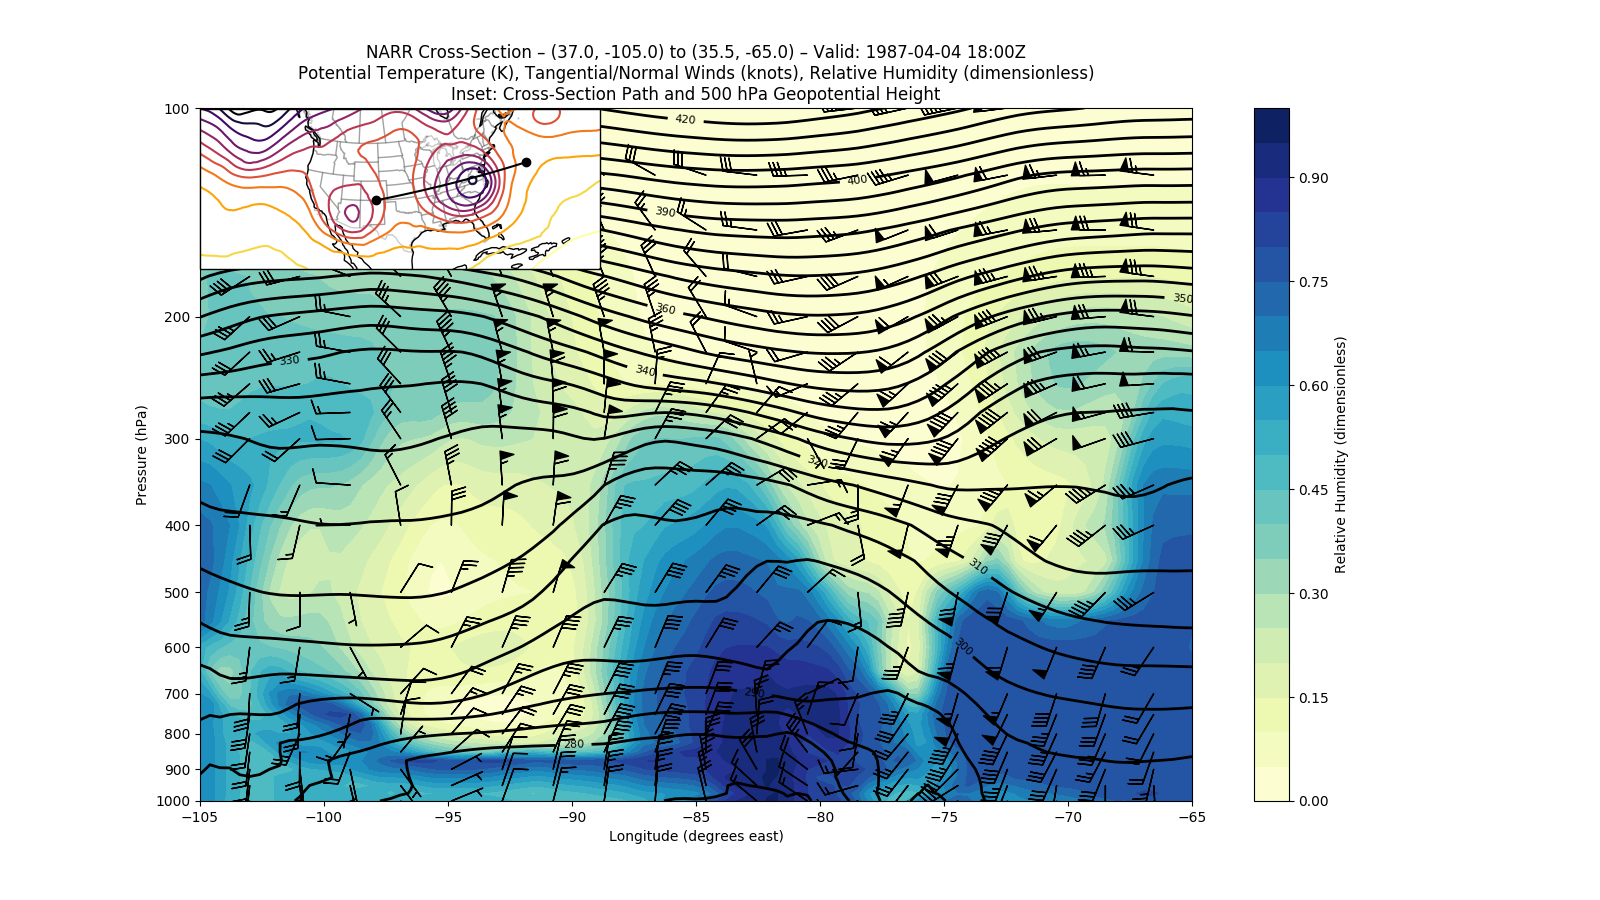
\includegraphics{sphx_glr_cross_section_001.png}

    So trying to replace: \includegraphics{./us-trenberth.gif}

    With: 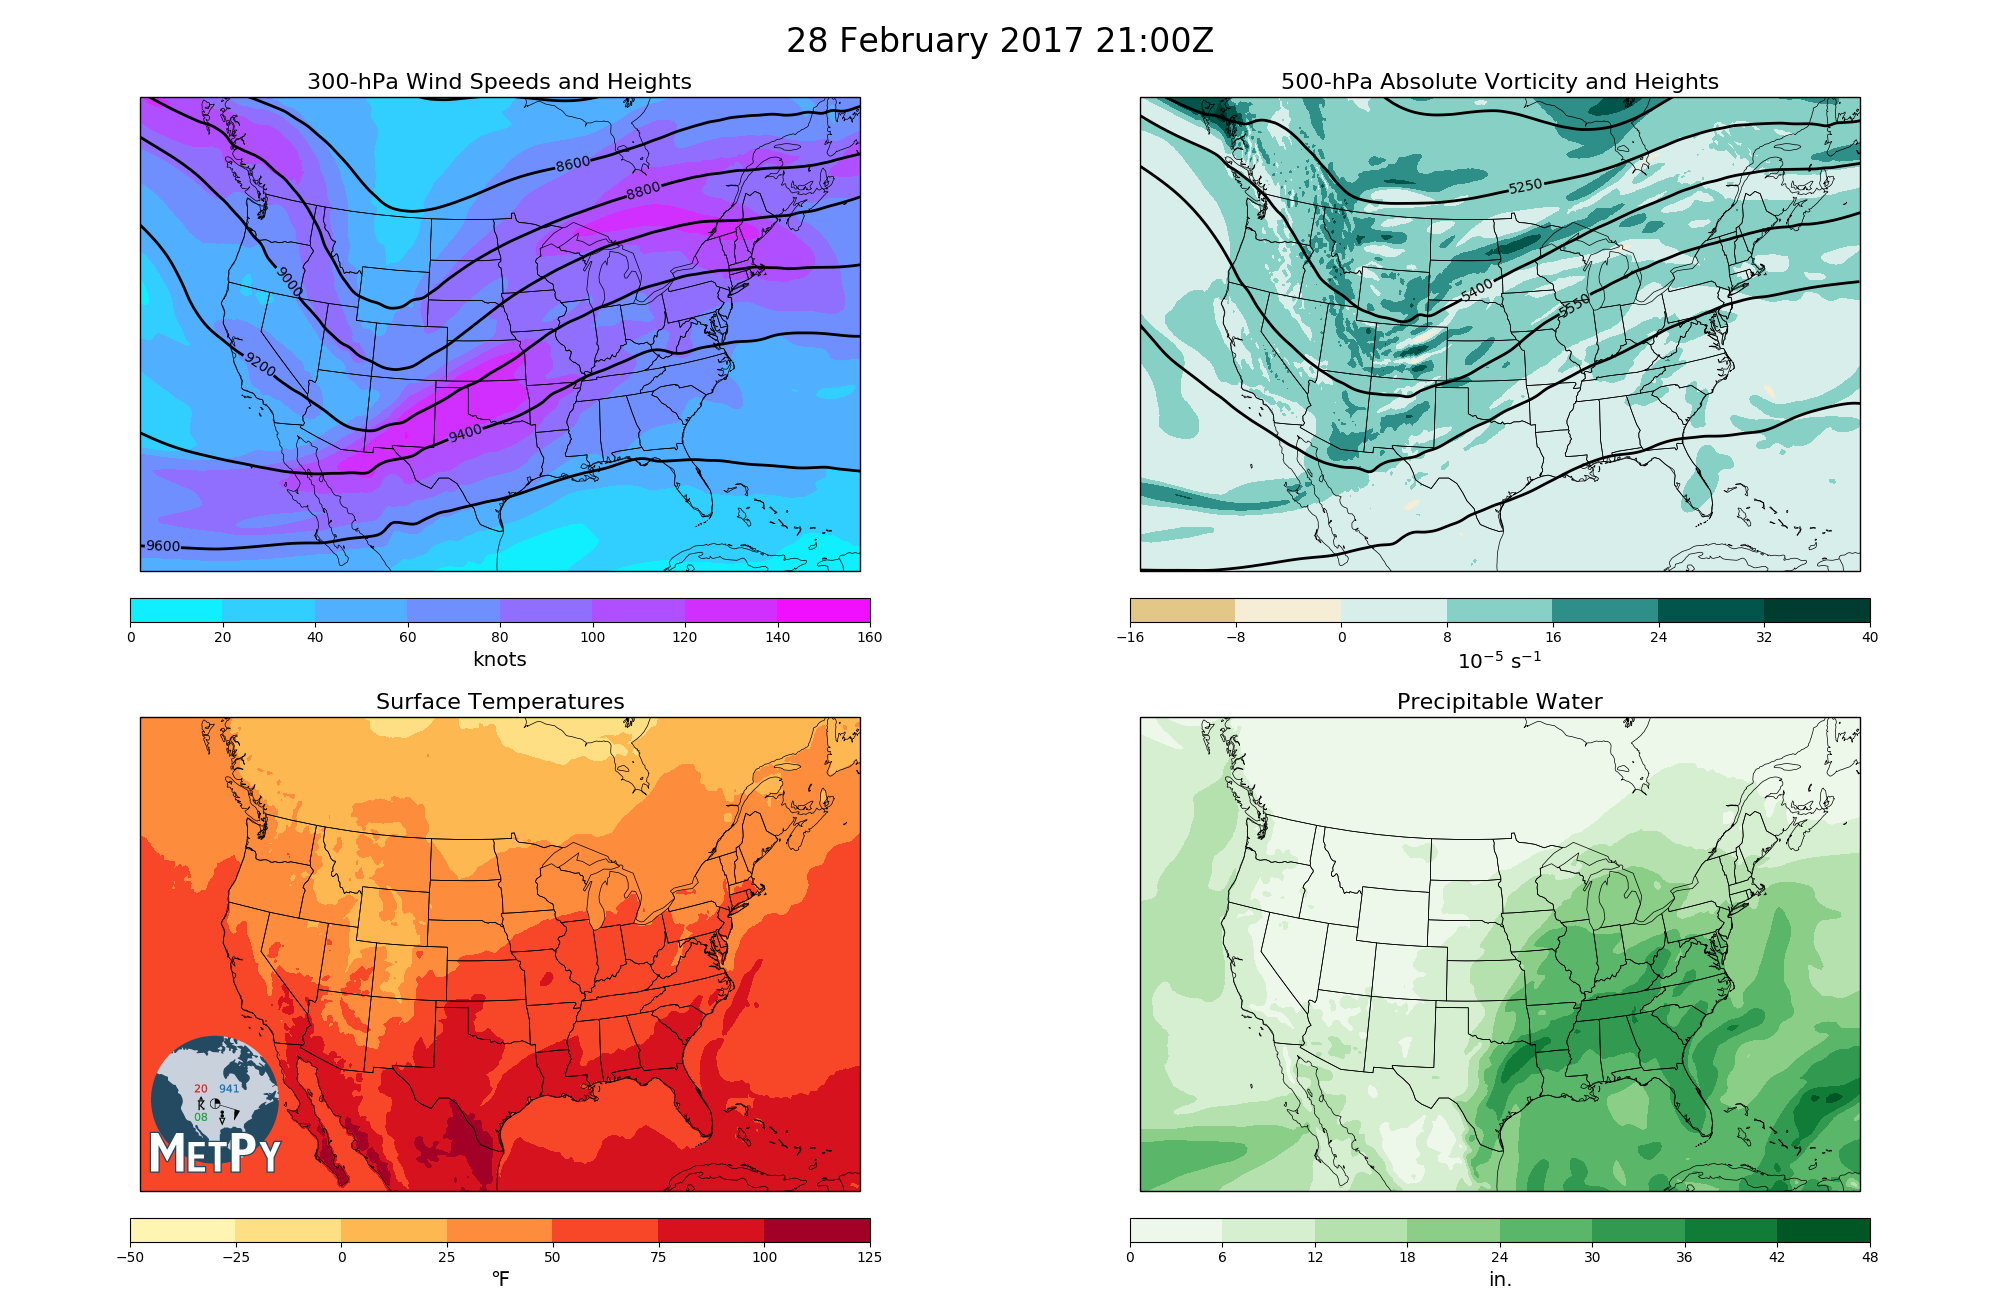
\includegraphics{./weather-map.png}

    \begin{itemize}
\tightlist
\item
  MetPy needs a data model for gridded data
\item
  Started using netCDF4-python
\item
  And adding stuff
\end{itemize}

    \begin{itemize}
\tightlist
\item
  This is pretty much XArray, so let's use it!
\end{itemize}

    \hypertarget{problem-1-projections}{%
\subsection{Problem 1: Projections}\label{problem-1-projections}}

\begin{itemize}
\tightlist
\item
  Assuming we have netCDF data, gridded coordinate systems store as a
  bundle of attributes
\item
  GOOD: Data are self-describing
\item
  BAD: Users have to convert these attributes into API calls (terrible
  for teaching)
\item
  Also, doing this generically is hard
\end{itemize}

    \begin{Verbatim}[commandchars=\\\{\}]
{\color{incolor}In [{\color{incolor}15}]:} \PY{n}{goes\PYZus{}cat} \PY{o}{=} \PY{n}{TDSCatalog}\PY{p}{(}\PY{l+s+s1}{\PYZsq{}}\PY{l+s+s1}{http://thredds\PYZhy{}test.unidata.ucar.edu/thredds/catalog/satellite/goes16/}\PY{l+s+s1}{\PYZsq{}}
                               \PY{l+s+s1}{\PYZsq{}}\PY{l+s+s1}{GOES16/CONUS/Channel14/current/catalog.xml}\PY{l+s+s1}{\PYZsq{}}\PY{p}{)}\PY{n}{w}
         \PY{n}{satdata} \PY{o}{=} \PY{n}{xr}\PY{o}{.}\PY{n}{open\PYZus{}dataset}\PY{p}{(}\PY{n}{goes\PYZus{}cat}\PY{o}{.}\PY{n}{datasets}\PY{p}{[}\PY{o}{\PYZhy{}}\PY{l+m+mi}{1}\PY{p}{]}\PY{o}{.}\PY{n}{access\PYZus{}urls}\PY{p}{[}\PY{l+s+s1}{\PYZsq{}}\PY{l+s+s1}{OPENDAP}\PY{l+s+s1}{\PYZsq{}}\PY{p}{]}\PY{p}{)}
         \PY{n}{proj\PYZus{}info} \PY{o}{=} \PY{n}{satdata}\PY{o}{.}\PY{n}{fixedgrid\PYZus{}projection}
         \PY{n}{proj\PYZus{}info}
\end{Verbatim}


\begin{Verbatim}[commandchars=\\\{\}]
{\color{outcolor}Out[{\color{outcolor}15}]:} <xarray.DataArray 'fixedgrid\_projection' ()>
         array(-2147483647, dtype=int32)
         Coordinates:
             time     datetime64[ns] {\ldots}
         Attributes:
             grid\_mapping\_name:               geostationary
             latitude\_of\_projection\_origin:   0.0
             longitude\_of\_projection\_origin:  -75.00000000000001
             semi\_major:                      6378137.0
             semi\_major\_axis:                 6378137.0
             semi\_minor:                      6356752.31414
             semi\_minor\_axis:                 6356752.31414
             perspective\_point\_height:        35785831.0
             sweep\_angle\_axis:                x
\end{Verbatim}
            
    \begin{Verbatim}[commandchars=\\\{\}]
{\color{incolor}In [{\color{incolor}12}]:} \PY{n}{fig} \PY{o}{=} \PY{n}{plt}\PY{o}{.}\PY{n}{figure}\PY{p}{(}\PY{n}{figsize}\PY{o}{=}\PY{p}{(}\PY{l+m+mi}{15}\PY{p}{,} \PY{l+m+mi}{10}\PY{p}{)}\PY{p}{)}
         \PY{n}{globe} \PY{o}{=} \PY{n}{ccrs}\PY{o}{.}\PY{n}{Globe}\PY{p}{(}\PY{n}{semimajor\PYZus{}axis}\PY{o}{=}\PY{n}{proj\PYZus{}info}\PY{o}{.}\PY{n}{semi\PYZus{}major\PYZus{}axis}\PY{p}{,}
                            \PY{n}{semiminor\PYZus{}axis}\PY{o}{=}\PY{n}{proj\PYZus{}info}\PY{o}{.}\PY{n}{semi\PYZus{}minor\PYZus{}axis}\PY{p}{)}
         \PY{n}{proj} \PY{o}{=} \PY{n}{ccrs}\PY{o}{.}\PY{n}{Geostationary}\PY{p}{(}\PY{n}{central\PYZus{}longitude}\PY{o}{=}\PY{n}{proj\PYZus{}info}\PY{o}{.}\PY{n}{longitude\PYZus{}of\PYZus{}projection\PYZus{}origin}\PY{p}{,}
                                   \PY{n}{satellite\PYZus{}height}\PY{o}{=}\PY{n}{proj\PYZus{}info}\PY{o}{.}\PY{n}{perspective\PYZus{}point\PYZus{}height}\PY{p}{,}
                                   \PY{n}{globe}\PY{o}{=}\PY{n}{globe}\PY{p}{,} \PY{n}{sweep\PYZus{}axis}\PY{o}{=}\PY{n}{proj\PYZus{}info}\PY{o}{.}\PY{n}{sweep\PYZus{}angle\PYZus{}axis}\PY{p}{)}
         \PY{n}{ax} \PY{o}{=} \PY{n}{fig}\PY{o}{.}\PY{n}{add\PYZus{}subplot}\PY{p}{(}\PY{l+m+mi}{1}\PY{p}{,} \PY{l+m+mi}{1}\PY{p}{,} \PY{l+m+mi}{1}\PY{p}{,} \PY{n}{projection}\PY{o}{=}\PY{n}{proj}\PY{p}{)}
         \PY{n}{ax}\PY{o}{.}\PY{n}{coastlines}\PY{p}{(}\PY{n}{resolution}\PY{o}{=}\PY{l+s+s1}{\PYZsq{}}\PY{l+s+s1}{50m}\PY{l+s+s1}{\PYZsq{}}\PY{p}{)}
         \PY{n}{x} \PY{o}{=} \PY{n}{satdata}\PY{o}{.}\PY{n}{x} \PY{o}{*} \PY{n}{proj\PYZus{}info}\PY{o}{.}\PY{n}{perspective\PYZus{}point\PYZus{}height} \PY{o}{/} \PY{l+m+mf}{1e6} 
         \PY{n}{y} \PY{o}{=} \PY{n}{satdata}\PY{o}{.}\PY{n}{y} \PY{o}{*} \PY{n}{proj\PYZus{}info}\PY{o}{.}\PY{n}{perspective\PYZus{}point\PYZus{}height} \PY{o}{/} \PY{l+m+mf}{1e6}
         \PY{n}{ax}\PY{o}{.}\PY{n}{imshow}\PY{p}{(}\PY{n}{satdata}\PY{o}{.}\PY{n}{Sectorized\PYZus{}CMI}\PY{p}{,} \PY{n}{cmap}\PY{o}{=}\PY{l+s+s1}{\PYZsq{}}\PY{l+s+s1}{Greys}\PY{l+s+s1}{\PYZsq{}}\PY{p}{,} \PY{n}{origin}\PY{o}{=}\PY{l+s+s1}{\PYZsq{}}\PY{l+s+s1}{upper}\PY{l+s+s1}{\PYZsq{}}\PY{p}{,}
                   \PY{n}{extent}\PY{o}{=}\PY{p}{(}\PY{n}{x}\PY{o}{.}\PY{n}{min}\PY{p}{(}\PY{p}{)}\PY{p}{,} \PY{n}{x}\PY{o}{.}\PY{n}{max}\PY{p}{(}\PY{p}{)}\PY{p}{,} \PY{n}{y}\PY{o}{.}\PY{n}{min}\PY{p}{(}\PY{p}{)}\PY{p}{,} \PY{n}{y}\PY{o}{.}\PY{n}{max}\PY{p}{(}\PY{p}{)}\PY{p}{)}\PY{p}{)}
\end{Verbatim}


\begin{Verbatim}[commandchars=\\\{\}]
{\color{outcolor}Out[{\color{outcolor}12}]:} <matplotlib.image.AxesImage at 0x109788320>
\end{Verbatim}
            
    \begin{center}
    \adjustimage{max size={0.9\linewidth}{0.9\paperheight}}{output_11_1.png}
    \end{center}
    { \hspace*{\fill} \\}
    
    \hypertarget{solution}{%
\subsection{Solution}\label{solution}}

\begin{itemize}
\tightlist
\item
  MetPy custom accessor on \texttt{Dataset} and \texttt{DataArray}
\item
  Registry of code to generate CartoPy projections from CF-compliant
  Metadata
\item
  By hooking into \texttt{Dataset}, we can properly walk the metadata
\end{itemize}

    \begin{Verbatim}[commandchars=\\\{\}]
{\color{incolor}In [{\color{incolor}16}]:} \PY{n}{fig} \PY{o}{=} \PY{n}{plt}\PY{o}{.}\PY{n}{figure}\PY{p}{(}\PY{n}{figsize}\PY{o}{=}\PY{p}{(}\PY{l+m+mi}{15}\PY{p}{,} \PY{l+m+mi}{10}\PY{p}{)}\PY{p}{)}
         \PY{n}{data} \PY{o}{=} \PY{n}{satdata}\PY{o}{.}\PY{n}{metpy}\PY{o}{.}\PY{n}{parse\PYZus{}cf}\PY{p}{(}\PY{l+s+s1}{\PYZsq{}}\PY{l+s+s1}{Sectorized\PYZus{}CMI}\PY{l+s+s1}{\PYZsq{}}\PY{p}{)}
         \PY{n}{ax} \PY{o}{=} \PY{n}{fig}\PY{o}{.}\PY{n}{add\PYZus{}subplot}\PY{p}{(}\PY{l+m+mi}{1}\PY{p}{,} \PY{l+m+mi}{1}\PY{p}{,} \PY{l+m+mi}{1}\PY{p}{,} \PY{n}{projection}\PY{o}{=}\PY{n}{data}\PY{o}{.}\PY{n}{metpy}\PY{o}{.}\PY{n}{cartopy\PYZus{}crs}\PY{p}{)}
         \PY{n}{ax}\PY{o}{.}\PY{n}{coastlines}\PY{p}{(}\PY{n}{resolution}\PY{o}{=}\PY{l+s+s1}{\PYZsq{}}\PY{l+s+s1}{50m}\PY{l+s+s1}{\PYZsq{}}\PY{p}{)}
         \PY{n}{ax}\PY{o}{.}\PY{n}{imshow}\PY{p}{(}\PY{n}{satdata}\PY{o}{.}\PY{n}{Sectorized\PYZus{}CMI}\PY{p}{,} \PY{n}{cmap}\PY{o}{=}\PY{l+s+s1}{\PYZsq{}}\PY{l+s+s1}{Greys}\PY{l+s+s1}{\PYZsq{}}\PY{p}{,} \PY{n}{origin}\PY{o}{=}\PY{l+s+s1}{\PYZsq{}}\PY{l+s+s1}{upper}\PY{l+s+s1}{\PYZsq{}}\PY{p}{,}
                   \PY{n}{extent}\PY{o}{=}\PY{p}{(}\PY{n}{data}\PY{o}{.}\PY{n}{x}\PY{o}{.}\PY{n}{min}\PY{p}{(}\PY{p}{)}\PY{p}{,} \PY{n}{data}\PY{o}{.}\PY{n}{x}\PY{o}{.}\PY{n}{max}\PY{p}{(}\PY{p}{)}\PY{p}{,}
                           \PY{n}{data}\PY{o}{.}\PY{n}{y}\PY{o}{.}\PY{n}{min}\PY{p}{(}\PY{p}{)}\PY{p}{,} \PY{n}{data}\PY{o}{.}\PY{n}{y}\PY{o}{.}\PY{n}{max}\PY{p}{(}\PY{p}{)}\PY{p}{)}\PY{p}{)}
\end{Verbatim}


\begin{Verbatim}[commandchars=\\\{\}]
{\color{outcolor}Out[{\color{outcolor}16}]:} <matplotlib.image.AxesImage at 0x128b2f208>
\end{Verbatim}
            
    \begin{center}
    \adjustimage{max size={0.9\linewidth}{0.9\paperheight}}{output_13_1.png}
    \end{center}
    { \hspace*{\fill} \\}
    
    \hypertarget{problem-2-units-and-calculations}{%
\subsection{Problem 2: Units and
Calculations}\label{problem-2-units-and-calculations}}

\begin{itemize}
\tightlist
\item
  MetPy's calculations are unit-aware, using pint
\item
  pint independently wraps NumPy arrays
\item
  pint + XArray -\textgreater{} Boom!
\end{itemize}

    \hypertarget{solution-sort-of}{%
\subsection{Solution (sort of)}\label{solution-sort-of}}

\begin{itemize}
\tightlist
\item
  Add \texttt{unit\_array} attribute to MetPy accessor

  \begin{itemize}
  \tightlist
  \item
    Automatically generate pint-wrapped array from XArray
    \texttt{DataArray} and \texttt{units} attribute
  \item
    Provides hook to adjust units as needed
  \item
    Can also convert \texttt{DataArray} in-place
  \end{itemize}
\item
  Decorate MetPy calculation functions

  \begin{itemize}
  \tightlist
  \item
    Check for \texttt{DataArray}s passed in and convert
  \item
    Makes calculations ``just work''
  \item
    Does \textbf{NOT} return \texttt{DataArray}
  \end{itemize}
\end{itemize}

    \begin{Verbatim}[commandchars=\\\{\}]
{\color{incolor}In [{\color{incolor}4}]:} \PY{n}{gfs\PYZus{}cat} \PY{o}{=} \PY{n}{TDSCatalog}\PY{p}{(}\PY{l+s+s1}{\PYZsq{}}\PY{l+s+s1}{http://thredds.ucar.edu/thredds/catalog/}\PY{l+s+s1}{\PYZsq{}}
                             \PY{l+s+s1}{\PYZsq{}}\PY{l+s+s1}{grib/NCEP/GFS/Global\PYZus{}0p5deg/catalog.xml}\PY{l+s+s1}{\PYZsq{}}\PY{p}{)}
        \PY{n}{gfs\PYZus{}data} \PY{o}{=} \PY{n}{xr}\PY{o}{.}\PY{n}{open\PYZus{}dataset}\PY{p}{(}\PY{n}{gfs\PYZus{}cat}\PY{o}{.}\PY{n}{latest}\PY{o}{.}\PY{n}{access\PYZus{}urls}\PY{p}{[}\PY{l+s+s1}{\PYZsq{}}\PY{l+s+s1}{OPENDAP}\PY{l+s+s1}{\PYZsq{}}\PY{p}{]}\PY{p}{)}
        \PY{n}{gfs\PYZus{}data}\PY{o}{.}\PY{n}{Relative\PYZus{}humidity\PYZus{}isobaric}\PY{o}{.}\PY{n}{attrs}\PY{p}{[}\PY{l+s+s1}{\PYZsq{}}\PY{l+s+s1}{units}\PY{l+s+s1}{\PYZsq{}}\PY{p}{]} \PY{o}{=} \PY{l+s+s1}{\PYZsq{}}\PY{l+s+s1}{percent}\PY{l+s+s1}{\PYZsq{}}
        \PY{n}{dewpt} \PY{o}{=} \PY{n}{mpcalc}\PY{o}{.}\PY{n}{dewpoint\PYZus{}rh}\PY{p}{(}
            \PY{n}{gfs\PYZus{}data}\PY{o}{.}\PY{n}{Temperature\PYZus{}isobaric}\PY{o}{.}\PY{n}{sel}\PY{p}{(}\PY{n}{isobaric}\PY{o}{=}\PY{l+m+mi}{50000}\PY{p}{)}\PY{p}{,}
            \PY{n}{gfs\PYZus{}data}\PY{o}{.}\PY{n}{Relative\PYZus{}humidity\PYZus{}isobaric}\PY{o}{.}\PY{n}{sel}\PY{p}{(}\PY{n}{isobaric}\PY{o}{=}\PY{l+m+mi}{50000}\PY{p}{)}\PY{p}{)}
\end{Verbatim}


    \begin{Verbatim}[commandchars=\\\{\}]
/Users/rmay/repos/metpy/metpy/calc/thermo.py:619: RuntimeWarning: overflow encountered in exp
  (temperature - 29.65 * units.kelvin))
/Users/rmay/miniconda3/envs/py36/lib/python3.6/site-packages/pint/quantity.py:1403: RuntimeWarning: overflow encountered in exp
  out = uf(*mobjs)
/Users/rmay/miniconda3/envs/py36/lib/python3.6/site-packages/pint/quantity.py:802: RuntimeWarning: invalid value encountered in multiply
  magnitude = magnitude\_op(new\_self.\_magnitude, other.\_magnitude)

    \end{Verbatim}

    \begin{itemize}
\tightlist
\item
  Good interim step
\item
  Allows starting to use XArray easily (we still need to make releases)
\item
  Half of the desired behavior
\end{itemize}

    \hypertarget{problem-3-dimension-names}{%
\section{Problem 3: Dimension Names}\label{problem-3-dimension-names}}

\begin{itemize}
\tightlist
\item
  THREDDS Data Server provides nice collections on top of GRIB files
\item
  Nature of GRIB makes this\ldots{}challenging to deal with:
\end{itemize}

    \begin{Verbatim}[commandchars=\\\{\}]
{\color{incolor}In [{\color{incolor}32}]:} \PY{n}{gfs\PYZus{}data} \PY{o}{=} \PY{n}{xr}\PY{o}{.}\PY{n}{open\PYZus{}dataset}\PY{p}{(}\PY{n}{gfs\PYZus{}cat}\PY{o}{.}\PY{n}{datasets}\PY{p}{[}\PY{l+m+mi}{1}\PY{p}{]}\PY{o}{.}\PY{n}{access\PYZus{}urls}\PY{p}{[}\PY{l+s+s1}{\PYZsq{}}\PY{l+s+s1}{OPENDAP}\PY{l+s+s1}{\PYZsq{}}\PY{p}{]}\PY{p}{)}
         \PY{n+nb}{print}\PY{p}{(}\PY{p}{[}\PY{n}{d} \PY{k}{for} \PY{n}{d} \PY{o+ow}{in} \PY{n}{gfs\PYZus{}data}\PY{o}{.}\PY{n}{dims} \PY{k}{if} \PY{l+s+s1}{\PYZsq{}}\PY{l+s+s1}{isobaric}\PY{l+s+s1}{\PYZsq{}} \PY{o+ow}{in} \PY{n}{d}\PY{p}{]}\PY{p}{)}
\end{Verbatim}


    \begin{Verbatim}[commandchars=\\\{\}]
['isobaric', 'isobaric1', 'isobaric2', 'isobaric3', 'isobaric4', 'isobaric5']

    \end{Verbatim}

    \begin{Verbatim}[commandchars=\\\{\}]
{\color{incolor}In [{\color{incolor}41}]:} \PY{n}{heights} \PY{o}{=} \PY{n}{gfs\PYZus{}data}\PY{o}{.}\PY{n}{metpy}\PY{o}{.}\PY{n}{parse\PYZus{}cf}\PY{p}{(}\PY{l+s+s1}{\PYZsq{}}\PY{l+s+s1}{Absolute\PYZus{}vorticity\PYZus{}isobaric}\PY{l+s+s1}{\PYZsq{}}\PY{p}{)}
         \PY{n}{heights}\PY{o}{.}\PY{n}{dims}
\end{Verbatim}


\begin{Verbatim}[commandchars=\\\{\}]
{\color{outcolor}Out[{\color{outcolor}41}]:} ('time', 'isobaric4', 'lat', 'lon')
\end{Verbatim}
            
    \hypertarget{solution-interpret-cf-metadata}{%
\subsection{Solution: Interpret CF
metadata}\label{solution-interpret-cf-metadata}}

    \begin{Verbatim}[commandchars=\\\{\}]
{\color{incolor}In [{\color{incolor}44}]:} \PY{n}{heights}\PY{o}{.}\PY{n}{metpy}\PY{o}{.}\PY{n}{vertical}
\end{Verbatim}


\begin{Verbatim}[commandchars=\\\{\}]
{\color{outcolor}Out[{\color{outcolor}44}]:} <xarray.DataArray 'isobaric4' (isobaric4: 26)>
         array([  1000.,   2000.,   3000.,   5000.,   7000.,  10000.,  15000.,  20000.,
                 25000.,  30000.,  35000.,  40000.,  45000.,  50000.,  55000.,  60000.,
                 65000.,  70000.,  75000.,  80000.,  85000.,  90000.,  92500.,  95000.,
                 97500., 100000.], dtype=float32)
         Coordinates:
           * isobaric4  (isobaric4) float32 1000.0 2000.0 3000.0 5000.0 7000.0 {\ldots}
             crs        object Projection: latitude\_longitude
         Attributes:
             units:                   Pa
             long\_name:               Isobaric surface
             positive:                down
             Grib\_level\_type:         100
             \_CoordinateAxisType:     Pressure
             \_CoordinateZisPositive:  down
             axis:                    Z
\end{Verbatim}
            
    \begin{itemize}
\tightlist
\item
  Will be released later this month in 0.9
\item
  Still kicking the tires on this to see if this is a good API
\item
  Used to power our cross-section support
\end{itemize}

    \hypertarget{future-work}{%
\subsection{Future work}\label{future-work}}

\begin{itemize}
\tightlist
\item
  So far using XArray is good
\end{itemize}

    \begin{itemize}
\tightlist
\item
  Except when it's not
\end{itemize}

    \hypertarget{more-problems-xarray-hates-tds}{%
\subsection{More Problems: XArray hates
TDS}\label{more-problems-xarray-hates-tds}}

    \hypertarget{full-collection}{%
\subsubsection{Full Collection}\label{full-collection}}

    \begin{Verbatim}[commandchars=\\\{\}]
{\color{incolor}In [{\color{incolor}51}]:} \PY{k}{try}\PY{p}{:}
             \PY{n}{xr}\PY{o}{.}\PY{n}{open\PYZus{}dataset}\PY{p}{(}\PY{n}{gfs\PYZus{}cat}\PY{o}{.}\PY{n}{datasets}\PY{p}{[}\PY{l+m+mi}{0}\PY{p}{]}\PY{o}{.}\PY{n}{access\PYZus{}urls}\PY{p}{[}\PY{l+s+s1}{\PYZsq{}}\PY{l+s+s1}{OPENDAP}\PY{l+s+s1}{\PYZsq{}}\PY{p}{]}\PY{p}{)}
         \PY{k}{except} \PY{n+ne}{Exception} \PY{k}{as} \PY{n}{e}\PY{p}{:}
             \PY{n+nb}{print}\PY{p}{(}\PY{n}{e}\PY{p}{)}
\end{Verbatim}


    \begin{Verbatim}[commandchars=\\\{\}]
'time' has more than 1-dimension and the same name as one of its dimensions ('reftime', 'time'). xarray disallows such variables because they conflict with the coordinates used to label dimensions.

    \end{Verbatim}

    \hypertarget{netcdf-subset-service}{%
\subsubsection{NetCDF Subset Service}\label{netcdf-subset-service}}

\begin{itemize}
\tightlist
\item
  TDS can subset a grid--this works well
\item
  TDS can also return point data (e.g.~timeseries) from the grid--this
  works\ldots{}not at all
\end{itemize}

    \begin{Verbatim}[commandchars=\\\{\}]
{\color{incolor}In [{\color{incolor}11}]:} \PY{k}{try}\PY{p}{:}
             \PY{n}{ncss} \PY{o}{=} \PY{n}{gfs\PYZus{}cat}\PY{o}{.}\PY{n}{latest}\PY{o}{.}\PY{n}{subset}\PY{p}{(}\PY{p}{)}
             \PY{n}{query} \PY{o}{=} \PY{n}{ncss}\PY{o}{.}\PY{n}{query}\PY{p}{(}\PY{p}{)}\PY{o}{.}\PY{n}{variables}\PY{p}{(}\PY{l+s+s1}{\PYZsq{}}\PY{l+s+s1}{Geopotential\PYZus{}height\PYZus{}isobaric}\PY{l+s+s1}{\PYZsq{}}\PY{p}{)}
             \PY{n}{query}\PY{o}{.}\PY{n}{time}\PY{p}{(}\PY{n}{datetime}\PY{o}{.}\PY{n}{utcnow}\PY{p}{(}\PY{p}{)}\PY{p}{)}\PY{o}{.}\PY{n}{lonlat\PYZus{}point}\PY{p}{(}\PY{n}{lon}\PY{o}{=}\PY{o}{\PYZhy{}}\PY{l+m+mi}{105}\PY{p}{,} \PY{n}{lat}\PY{o}{=}\PY{l+m+mi}{40}\PY{p}{)}
             \PY{n}{query}\PY{o}{.}\PY{n}{add\PYZus{}lonlat}\PY{p}{(}\PY{p}{)}\PY{o}{.}\PY{n}{accept}\PY{p}{(}\PY{l+s+s1}{\PYZsq{}}\PY{l+s+s1}{netcdf4}\PY{l+s+s1}{\PYZsq{}}\PY{p}{)}
             \PY{n}{nc} \PY{o}{=} \PY{n}{ncss}\PY{o}{.}\PY{n}{get\PYZus{}data}\PY{p}{(}\PY{n}{query}\PY{p}{)}
             \PY{n}{xr}\PY{o}{.}\PY{n}{open\PYZus{}dataset}\PY{p}{(}\PY{n}{NetCDF4DataStore}\PY{p}{(}\PY{n}{nc}\PY{p}{)}\PY{p}{)}
         \PY{k}{except} \PY{n+ne}{Exception} \PY{k}{as} \PY{n}{e}\PY{p}{:}
             \PY{n+nb}{print}\PY{p}{(}\PY{n+nb}{str}\PY{p}{(}\PY{n}{e}\PY{p}{)}\PY{p}{)}
\end{Verbatim}


    \begin{Verbatim}[commandchars=\\\{\}]
'isobaric' has more than 1-dimension and the same name as one of its dimensions ('station', 'profile', 'isobaric'). xarray disallows such variables because they conflict with the coordinates used to label dimensions.

    \end{Verbatim}

    \hypertarget{units}{%
\subsection{Units}\label{units}}

\begin{figure}
\centering
\includegraphics{./perry-headsmash.gif}
\caption{Head Smash}
\end{figure}

    \begin{figure}
\centering
\includegraphics{./good-tire-fire.gif}
\caption{Tire Fire}
\end{figure}

    \begin{itemize}
\tightlist
\item
  Making multiple numpy array subclasses (or array-like) play together
  is \sout{impossible} really hard
\item
  There's movement in the community\ldots{}but it's slow
\item
  I had been focused on getting XArray to wrap a pint array\ldots{}
\item
  I think the best approach are hooks in XArray, maybe in
  \texttt{\_\_array\_ufunc\_\_}
\item
  Tightly coupled into XArray\ldots{}maybe using cf\_units/udunits?
\item
  Any other thoughts?
\end{itemize}

    \begin{Verbatim}[commandchars=\\\{\}]
{\color{incolor}In [{\color{incolor}64}]:} \PY{o}{\PYZpc{}}\PY{k}{matplotlib} inline
         \PY{k+kn}{from} \PY{n+nn}{datetime} \PY{k}{import} \PY{n}{datetime}
         \PY{k+kn}{from} \PY{n+nn}{traitlets} \PY{k}{import} \PY{n}{HasTraits}\PY{p}{,} \PY{n}{Unicode}\PY{p}{,} \PY{n}{Tuple}\PY{p}{,} \PY{n}{Int}\PY{p}{,} \PY{n}{List}\PY{p}{,} \PY{n}{Any}\PY{p}{,} \PY{n}{Union}\PY{p}{,} \PY{n}{Instance}\PY{p}{,} \PY{n}{Float}\PY{p}{,} \PY{n}{default}\PY{p}{,} \PY{n}{observe}\PY{p}{,} \PY{n}{link}
         \PY{k+kn}{import} \PY{n+nn}{cartopy}\PY{n+nn}{.}\PY{n+nn}{crs} \PY{k}{as} \PY{n+nn}{ccrs}
         \PY{k+kn}{import} \PY{n+nn}{cartopy}\PY{n+nn}{.}\PY{n+nn}{feature} \PY{k}{as} \PY{n+nn}{cfeat}
         \PY{k+kn}{import} \PY{n+nn}{matplotlib}\PY{n+nn}{.}\PY{n+nn}{pyplot} \PY{k}{as} \PY{n+nn}{plt}
         \PY{k+kn}{import} \PY{n+nn}{numpy} \PY{k}{as} \PY{n+nn}{np}
         \PY{k+kn}{from} \PY{n+nn}{metpy}\PY{n+nn}{.}\PY{n+nn}{cbook} \PY{k}{import} \PY{n}{is\PYZus{}string\PYZus{}like}
         \PY{k+kn}{from} \PY{n+nn}{metpy}\PY{n+nn}{.}\PY{n+nn}{plots} \PY{k}{import} \PY{n}{ctables}
         
         \PY{n}{proj\PYZus{}lookup} \PY{o}{=} \PY{n+nb}{dict}\PY{p}{(}\PY{n}{lcc}\PY{o}{=}\PY{n}{ccrs}\PY{o}{.}\PY{n}{LambertConformal}\PY{p}{(}\PY{n}{central\PYZus{}latitude}\PY{o}{=}\PY{l+m+mi}{40}\PY{p}{,} \PY{n}{central\PYZus{}longitude}\PY{o}{=}\PY{o}{\PYZhy{}}\PY{l+m+mi}{100}\PY{p}{,}
                                                      \PY{n}{standard\PYZus{}parallels}\PY{o}{=}\PY{p}{[}\PY{l+m+mi}{30}\PY{p}{,} \PY{l+m+mi}{60}\PY{p}{]}\PY{p}{)}\PY{p}{)}
         \PY{n}{garea\PYZus{}lookup} \PY{o}{=} \PY{n+nb}{dict}\PY{p}{(}\PY{n}{us}\PY{o}{=}\PY{p}{(}\PY{o}{\PYZhy{}}\PY{l+m+mi}{115}\PY{p}{,} \PY{o}{\PYZhy{}}\PY{l+m+mi}{65}\PY{p}{,} \PY{l+m+mi}{25}\PY{p}{,} \PY{l+m+mi}{50}\PY{p}{)}\PY{p}{)}
         
         \PY{k}{class} \PY{n+nc}{Map}\PY{p}{(}\PY{n}{HasTraits}\PY{p}{)}\PY{p}{:}
             \PY{n}{garea} \PY{o}{=} \PY{n}{Unicode}\PY{p}{(}\PY{p}{)}
             \PY{n}{proj} \PY{o}{=} \PY{n}{Union}\PY{p}{(}\PY{p}{[}\PY{n}{Unicode}\PY{p}{(}\PY{p}{)}\PY{p}{,} \PY{n}{Instance}\PY{p}{(}\PY{n}{ccrs}\PY{o}{.}\PY{n}{Projection}\PY{p}{)}\PY{p}{]}\PY{p}{)}
             \PY{n}{plots} \PY{o}{=} \PY{n}{List}\PY{p}{(}\PY{n}{Any}\PY{p}{(}\PY{p}{)}\PY{p}{)}
             \PY{n}{figsize} \PY{o}{=} \PY{n}{Tuple}\PY{p}{(}\PY{n}{Int}\PY{p}{(}\PY{p}{)}\PY{p}{,} \PY{n}{Int}\PY{p}{(}\PY{p}{)}\PY{p}{)}
             \PY{n}{layout} \PY{o}{=} \PY{n}{Tuple}\PY{p}{(}\PY{n}{Int}\PY{p}{(}\PY{p}{)}\PY{p}{,} \PY{n}{Int}\PY{p}{(}\PY{p}{)}\PY{p}{)}
             
             \PY{n+nd}{@default}\PY{p}{(}\PY{l+s+s1}{\PYZsq{}}\PY{l+s+s1}{layout}\PY{l+s+s1}{\PYZsq{}}\PY{p}{)}
             \PY{k}{def} \PY{n+nf}{default\PYZus{}layout}\PY{p}{(}\PY{n+nb+bp}{self}\PY{p}{)}\PY{p}{:}
                 \PY{k}{return} \PY{p}{(}\PY{l+m+mi}{1}\PY{p}{,} \PY{l+m+mi}{1}\PY{p}{)}
         
             \PY{n+nd}{@observe}\PY{p}{(}\PY{l+s+s1}{\PYZsq{}}\PY{l+s+s1}{plots}\PY{l+s+s1}{\PYZsq{}}\PY{p}{)}
             \PY{k}{def} \PY{n+nf}{\PYZus{}plots\PYZus{}changed}\PY{p}{(}\PY{n+nb+bp}{self}\PY{p}{,} \PY{n}{change}\PY{p}{)}\PY{p}{:}
                 \PY{k}{if} \PY{n+nb}{hasattr}\PY{p}{(}\PY{n+nb+bp}{self}\PY{p}{,} \PY{l+s+s1}{\PYZsq{}}\PY{l+s+s1}{fig}\PY{l+s+s1}{\PYZsq{}}\PY{p}{)}\PY{p}{:}
                     \PY{n+nb}{delattr}\PY{p}{(}\PY{n+nb+bp}{self}\PY{p}{,} \PY{l+s+s1}{\PYZsq{}}\PY{l+s+s1}{fig}\PY{l+s+s1}{\PYZsq{}}\PY{p}{)}
                 \PY{k}{for} \PY{n}{plot} \PY{o+ow}{in} \PY{n}{change}\PY{o}{.}\PY{n}{new}\PY{p}{:}
                     \PY{n}{plot}\PY{o}{.}\PY{n}{observe}\PY{p}{(}\PY{n+nb+bp}{self}\PY{o}{.}\PY{n}{refresh}\PY{p}{)}
         
             \PY{k}{def} \PY{n+nf}{refresh}\PY{p}{(}\PY{n+nb+bp}{self}\PY{p}{,} \PY{n}{\PYZus{}}\PY{p}{)}\PY{p}{:}
                 \PY{n+nb+bp}{self}\PY{o}{.}\PY{n}{draw}\PY{p}{(}\PY{p}{)}
                 \PY{n+nb+bp}{self}\PY{o}{.}\PY{n}{fig}\PY{o}{.}\PY{n}{canvas}\PY{o}{.}\PY{n}{draw}\PY{p}{(}\PY{p}{)}
                 \PY{n+nb+bp}{self}\PY{o}{.}\PY{n}{fig}\PY{o}{.}\PY{n}{canvas}\PY{o}{.}\PY{n}{flush\PYZus{}events}\PY{p}{(}\PY{p}{)}
                 
             \PY{k}{def} \PY{n+nf}{draw}\PY{p}{(}\PY{n+nb+bp}{self}\PY{p}{)}\PY{p}{:}
                 \PY{k}{if} \PY{o+ow}{not} \PY{n+nb}{hasattr}\PY{p}{(}\PY{n+nb+bp}{self}\PY{p}{,} \PY{l+s+s1}{\PYZsq{}}\PY{l+s+s1}{fig}\PY{l+s+s1}{\PYZsq{}}\PY{p}{)}\PY{p}{:}
                     \PY{n+nb+bp}{self}\PY{o}{.}\PY{n}{fig} \PY{o}{=} \PY{n}{plt}\PY{o}{.}\PY{n}{figure}\PY{p}{(}\PY{n}{figsize}\PY{o}{=}\PY{n+nb+bp}{self}\PY{o}{.}\PY{n}{figsize}\PY{p}{)}
                     \PY{k}{if} \PY{n}{is\PYZus{}string\PYZus{}like}\PY{p}{(}\PY{n+nb+bp}{self}\PY{o}{.}\PY{n}{proj}\PY{p}{)}\PY{p}{:}
                         \PY{k}{if} \PY{n+nb+bp}{self}\PY{o}{.}\PY{n}{proj} \PY{o}{==} \PY{l+s+s1}{\PYZsq{}}\PY{l+s+s1}{data}\PY{l+s+s1}{\PYZsq{}}\PY{p}{:}
                             \PY{n}{proj} \PY{o}{=} \PY{n+nb+bp}{self}\PY{o}{.}\PY{n}{plots}\PY{p}{[}\PY{l+m+mi}{0}\PY{p}{]}\PY{o}{.}\PY{n}{griddata}\PY{o}{.}\PY{n}{metpy}\PY{o}{.}\PY{n}{cartopy\PYZus{}crs}
                         \PY{k}{else}\PY{p}{:}
                             \PY{n}{proj} \PY{o}{=} \PY{n}{proj\PYZus{}lookup}\PY{p}{[}\PY{n+nb+bp}{self}\PY{o}{.}\PY{n}{proj}\PY{p}{]}
                     \PY{k}{else}\PY{p}{:}
                         \PY{n}{proj} \PY{o}{=} \PY{n+nb+bp}{self}\PY{o}{.}\PY{n}{proj}
                     \PY{n}{nrow}\PY{p}{,} \PY{n}{ncol} \PY{o}{=} \PY{n+nb+bp}{self}\PY{o}{.}\PY{n}{layout}
                     \PY{n+nb+bp}{self}\PY{o}{.}\PY{n}{ax} \PY{o}{=} \PY{n+nb+bp}{self}\PY{o}{.}\PY{n}{fig}\PY{o}{.}\PY{n}{add\PYZus{}subplot}\PY{p}{(}\PY{n}{nrow}\PY{p}{,} \PY{n}{ncol}\PY{p}{,} \PY{l+m+mi}{1}\PY{p}{,} \PY{n}{projection}\PY{o}{=}\PY{n}{proj}\PY{p}{)}
                 \PY{k}{else}\PY{p}{:}
                     \PY{n+nb+bp}{self}\PY{o}{.}\PY{n}{ax}\PY{o}{.}\PY{n}{cla}\PY{p}{(}\PY{p}{)}
         
                 \PY{k}{for} \PY{n}{p} \PY{o+ow}{in} \PY{n+nb+bp}{self}\PY{o}{.}\PY{n}{plots}\PY{p}{:}
                     \PY{n}{p}\PY{o}{.}\PY{n}{draw}\PY{p}{(}\PY{n+nb+bp}{self}\PY{o}{.}\PY{n}{ax}\PY{p}{)}        
         
                 \PY{n+nb+bp}{self}\PY{o}{.}\PY{n}{ax}\PY{o}{.}\PY{n}{coastlines}\PY{p}{(}\PY{l+s+s1}{\PYZsq{}}\PY{l+s+s1}{50m}\PY{l+s+s1}{\PYZsq{}}\PY{p}{,} \PY{n}{zorder}\PY{o}{=}\PY{l+m+mi}{20}\PY{p}{)}
                 \PY{n+nb+bp}{self}\PY{o}{.}\PY{n}{ax}\PY{o}{.}\PY{n}{add\PYZus{}feature}\PY{p}{(}\PY{n}{cfeat}\PY{o}{.}\PY{n}{STATES}\PY{p}{,} \PY{n}{zorder}\PY{o}{=}\PY{l+m+mi}{20}\PY{p}{)}
         
                 \PY{k}{if} \PY{n+nb+bp}{self}\PY{o}{.}\PY{n}{garea}\PY{p}{:}
                     \PY{k}{if} \PY{n+nb+bp}{self}\PY{o}{.}\PY{n}{garea} \PY{o}{==} \PY{l+s+s1}{\PYZsq{}}\PY{l+s+s1}{global}\PY{l+s+s1}{\PYZsq{}}\PY{p}{:}
                         \PY{n+nb+bp}{self}\PY{o}{.}\PY{n}{ax}\PY{o}{.}\PY{n}{set\PYZus{}global}\PY{p}{(}\PY{p}{)}
                     \PY{k}{else}\PY{p}{:}
                         \PY{n+nb+bp}{self}\PY{o}{.}\PY{n}{ax}\PY{o}{.}\PY{n}{set\PYZus{}extent}\PY{p}{(}\PY{n}{garea\PYZus{}lookup}\PY{p}{[}\PY{n+nb+bp}{self}\PY{o}{.}\PY{n}{garea}\PY{p}{]}\PY{p}{,} \PY{n}{ccrs}\PY{o}{.}\PY{n}{PlateCarree}\PY{p}{(}\PY{p}{)}\PY{p}{)}
                 
                 \PY{n+nb+bp}{self}\PY{o}{.}\PY{n}{ax}\PY{o}{.}\PY{n}{set\PYZus{}title}\PY{p}{(}\PY{l+s+s1}{\PYZsq{}}\PY{l+s+s1}{, }\PY{l+s+s1}{\PYZsq{}}\PY{o}{.}\PY{n}{join}\PY{p}{(}\PY{n}{plot}\PY{o}{.}\PY{n}{name} \PY{k}{for} \PY{n}{plot} \PY{o+ow}{in} \PY{n+nb+bp}{self}\PY{o}{.}\PY{n}{plots}\PY{p}{)}\PY{p}{)}
                 \PY{k}{return} \PY{n+nb+bp}{self}\PY{o}{.}\PY{n}{fig}
         
             \PY{k}{def} \PY{n+nf}{\PYZus{}\PYZus{}getitem\PYZus{}\PYZus{}}\PY{p}{(}\PY{n+nb+bp}{self}\PY{p}{,} \PY{n}{ind}\PY{p}{)}\PY{p}{:}
                 \PY{c+c1}{\PYZsh{} TODO: Return particular axes}
                 \PY{k}{pass}
         
         \PY{k}{class} \PY{n+nc}{Plot}\PY{p}{(}\PY{n}{HasTraits}\PY{p}{)}\PY{p}{:}
         \PY{c+c1}{\PYZsh{}    data = Any()}
         \PY{c+c1}{\PYZsh{}    data = Instance(xr.Dataset)}
             \PY{n}{gfunc} \PY{o}{=} \PY{n}{Unicode}\PY{p}{(}\PY{p}{)}
             \PY{n}{glevel} \PY{o}{=} \PY{n}{Int}\PY{p}{(}\PY{n}{allow\PYZus{}none}\PY{o}{=}\PY{k+kc}{True}\PY{p}{,} \PY{n}{default\PYZus{}value}\PY{o}{=}\PY{k+kc}{None}\PY{p}{)}
             \PY{n}{data\PYZus{}time} \PY{o}{=} \PY{n}{Instance}\PY{p}{(}\PY{n}{datetime}\PY{p}{,} \PY{n}{allow\PYZus{}none}\PY{o}{=}\PY{k+kc}{True}\PY{p}{)}
         
             \PY{n+nd}{@observe}\PY{p}{(}\PY{l+s+s1}{\PYZsq{}}\PY{l+s+s1}{gfunc}\PY{l+s+s1}{\PYZsq{}}\PY{p}{)}
             \PY{k}{def} \PY{n+nf}{\PYZus{}update\PYZus{}data}\PY{p}{(}\PY{n+nb+bp}{self}\PY{p}{,} \PY{n}{changed}\PY{p}{)}\PY{p}{:}
                 \PY{n+nb+bp}{self}\PY{o}{.}\PY{n}{\PYZus{}griddata} \PY{o}{=} \PY{n+nb+bp}{self}\PY{o}{.}\PY{n}{data}\PY{o}{.}\PY{n}{metpy}\PY{o}{.}\PY{n}{parse\PYZus{}cf}\PY{p}{(}\PY{n}{changed}\PY{o}{.}\PY{n}{new}\PY{p}{)}
         
             \PY{n+nd}{@property}
             \PY{k}{def} \PY{n+nf}{griddata}\PY{p}{(}\PY{n+nb+bp}{self}\PY{p}{)}\PY{p}{:}
                 \PY{k}{return} \PY{n+nb+bp}{self}\PY{o}{.}\PY{n}{\PYZus{}griddata}
         
             \PY{n+nd}{@property}
             \PY{k}{def} \PY{n+nf}{plotdata}\PY{p}{(}\PY{n+nb+bp}{self}\PY{p}{)}\PY{p}{:}
                 \PY{n}{subset} \PY{o}{=} \PY{p}{\PYZob{}}\PY{l+s+s1}{\PYZsq{}}\PY{l+s+s1}{method}\PY{l+s+s1}{\PYZsq{}}\PY{p}{:} \PY{l+s+s1}{\PYZsq{}}\PY{l+s+s1}{nearest}\PY{l+s+s1}{\PYZsq{}}\PY{p}{\PYZcb{}}
                 \PY{k}{if} \PY{n+nb+bp}{self}\PY{o}{.}\PY{n}{glevel} \PY{o+ow}{is} \PY{o+ow}{not} \PY{k+kc}{None}\PY{p}{:}
                     \PY{n}{subset}\PY{p}{[}\PY{n+nb+bp}{self}\PY{o}{.}\PY{n}{griddata}\PY{o}{.}\PY{n}{metpy}\PY{o}{.}\PY{n}{vertical}\PY{o}{.}\PY{n}{name}\PY{p}{]} \PY{o}{=} \PY{n+nb+bp}{self}\PY{o}{.}\PY{n}{glevel}
         
                 \PY{k}{if} \PY{n+nb+bp}{self}\PY{o}{.}\PY{n}{data\PYZus{}time} \PY{o+ow}{is} \PY{o+ow}{not} \PY{k+kc}{None}\PY{p}{:}
                     \PY{n}{subset}\PY{p}{[}\PY{n+nb+bp}{self}\PY{o}{.}\PY{n}{griddata}\PY{o}{.}\PY{n}{metpy}\PY{o}{.}\PY{n}{time}\PY{o}{.}\PY{n}{name}\PY{p}{]} \PY{o}{=} \PY{n+nb+bp}{self}\PY{o}{.}\PY{n}{data\PYZus{}time}
         
                 \PY{n}{imdata} \PY{o}{=} \PY{n+nb+bp}{self}\PY{o}{.}\PY{n}{griddata}\PY{o}{.}\PY{n}{sel}\PY{p}{(}\PY{o}{*}\PY{o}{*}\PY{n}{subset}\PY{p}{)}
                 
                 \PY{n}{x} \PY{o}{=} \PY{n+nb+bp}{self}\PY{o}{.}\PY{n}{griddata}\PY{o}{.}\PY{n}{metpy}\PY{o}{.}\PY{n}{x}
                 \PY{n}{y} \PY{o}{=} \PY{n+nb+bp}{self}\PY{o}{.}\PY{n}{griddata}\PY{o}{.}\PY{n}{metpy}\PY{o}{.}\PY{n}{y}
                 \PY{k}{if} \PY{l+s+s1}{\PYZsq{}}\PY{l+s+s1}{degree}\PY{l+s+s1}{\PYZsq{}} \PY{o+ow}{in} \PY{n}{x}\PY{o}{.}\PY{n}{units}\PY{p}{:}
                     \PY{n}{X}\PY{p}{,} \PY{n}{Y} \PY{o}{=} \PY{n}{np}\PY{o}{.}\PY{n}{meshgrid}\PY{p}{(}\PY{n}{x}\PY{p}{,} \PY{n}{y}\PY{p}{)}
                     \PY{n}{x}\PY{p}{,} \PY{n}{y}\PY{p}{,} \PY{n}{\PYZus{}} \PY{o}{=} \PY{n+nb+bp}{self}\PY{o}{.}\PY{n}{griddata}\PY{o}{.}\PY{n}{metpy}\PY{o}{.}\PY{n}{cartopy\PYZus{}crs}\PY{o}{.}\PY{n}{transform\PYZus{}points}\PY{p}{(}\PY{n}{ccrs}\PY{o}{.}\PY{n}{PlateCarree}\PY{p}{(}\PY{p}{)}\PY{p}{,} \PY{n}{X}\PY{p}{,} \PY{n}{Y}\PY{p}{)}\PY{o}{.}\PY{n}{T}
                     \PY{n}{x} \PY{o}{=} \PY{n}{x}\PY{p}{[}\PY{p}{:}\PY{p}{,} \PY{l+m+mi}{0}\PY{p}{]} \PY{o}{\PYZpc{}} \PY{l+m+mi}{360}
                     \PY{n}{y} \PY{o}{=} \PY{n}{y}\PY{p}{[}\PY{l+m+mi}{0}\PY{p}{,} \PY{p}{:}\PY{p}{]}
                 
                 \PY{k}{return} \PY{n}{x}\PY{p}{,} \PY{n}{y}\PY{p}{,} \PY{n}{imdata}
         
             \PY{n+nd}{@property}
             \PY{k}{def} \PY{n+nf}{name}\PY{p}{(}\PY{n+nb+bp}{self}\PY{p}{)}\PY{p}{:}
                 \PY{n}{ret} \PY{o}{=} \PY{n+nb+bp}{self}\PY{o}{.}\PY{n}{gfunc}
                 \PY{k}{if} \PY{n+nb+bp}{self}\PY{o}{.}\PY{n}{glevel} \PY{o+ow}{is} \PY{o+ow}{not} \PY{k+kc}{None}\PY{p}{:}
                     \PY{n}{ret} \PY{o}{+}\PY{o}{=} \PY{l+s+s1}{\PYZsq{}}\PY{l+s+s1}{@}\PY{l+s+si}{\PYZob{}:d\PYZcb{}}\PY{l+s+s1}{\PYZsq{}}\PY{o}{.}\PY{n}{format}\PY{p}{(}\PY{n+nb+bp}{self}\PY{o}{.}\PY{n}{glevel}\PY{p}{)}
                 \PY{k}{return} \PY{n}{ret}
             
             \PY{n+nd}{@property}
             \PY{k}{def} \PY{n+nf}{code}\PY{p}{(}\PY{n+nb+bp}{self}\PY{p}{)}\PY{p}{:}
                 \PY{k}{pass}
         
         \PY{k}{class} \PY{n+nc}{ImagePlot}\PY{p}{(}\PY{n}{Plot}\PY{p}{)}\PY{p}{:}
             \PY{n}{ctable} \PY{o}{=} \PY{n}{Unicode}\PY{p}{(}\PY{p}{)}
             \PY{n}{img\PYZus{}range} \PY{o}{=} \PY{n}{Tuple}\PY{p}{(}\PY{n}{Int}\PY{p}{(}\PY{n}{allow\PYZus{}none}\PY{o}{=}\PY{k+kc}{True}\PY{p}{)}\PY{p}{,} \PY{n}{Int}\PY{p}{(}\PY{n}{allow\PYZus{}none}\PY{o}{=}\PY{k+kc}{True}\PY{p}{)}\PY{p}{)}
         
             \PY{n+nd}{@default}\PY{p}{(}\PY{l+s+s1}{\PYZsq{}}\PY{l+s+s1}{img\PYZus{}range}\PY{l+s+s1}{\PYZsq{}}\PY{p}{)}
             \PY{k}{def} \PY{n+nf}{default\PYZus{}img\PYZus{}range}\PY{p}{(}\PY{n+nb+bp}{self}\PY{p}{)}\PY{p}{:}
                 \PY{k}{return} \PY{k+kc}{None}\PY{p}{,} \PY{k+kc}{None}
         
             \PY{k}{def} \PY{n+nf}{draw}\PY{p}{(}\PY{n+nb+bp}{self}\PY{p}{,} \PY{n}{ax}\PY{p}{)}\PY{p}{:}
                 \PY{n}{x}\PY{p}{,} \PY{n}{y}\PY{p}{,} \PY{n}{imdata} \PY{o}{=} \PY{n+nb+bp}{self}\PY{o}{.}\PY{n}{plotdata}
         
                 \PY{n}{extents} \PY{o}{=} \PY{p}{(}\PY{n}{x}\PY{o}{.}\PY{n}{min}\PY{p}{(}\PY{p}{)}\PY{p}{,} \PY{n}{x}\PY{o}{.}\PY{n}{max}\PY{p}{(}\PY{p}{)}\PY{p}{,} \PY{n}{y}\PY{o}{.}\PY{n}{min}\PY{p}{(}\PY{p}{)}\PY{p}{,} \PY{n}{y}\PY{o}{.}\PY{n}{max}\PY{p}{(}\PY{p}{)}\PY{p}{)}
                 \PY{n}{origin} \PY{o}{=} \PY{l+s+s1}{\PYZsq{}}\PY{l+s+s1}{upper}\PY{l+s+s1}{\PYZsq{}} \PY{k}{if} \PY{n}{y}\PY{p}{[}\PY{l+m+mi}{0}\PY{p}{]} \PY{o}{\PYZgt{}} \PY{n}{y}\PY{p}{[}\PY{o}{\PYZhy{}}\PY{l+m+mi}{1}\PY{p}{]} \PY{k}{else} \PY{l+s+s1}{\PYZsq{}}\PY{l+s+s1}{lower}\PY{l+s+s1}{\PYZsq{}}
         
                 \PY{k}{try}\PY{p}{:}
                     \PY{n}{cmap} \PY{o}{=} \PY{n}{ctables}\PY{o}{.}\PY{n}{registry}\PY{o}{.}\PY{n}{get\PYZus{}colortable}\PY{p}{(}\PY{n+nb+bp}{self}\PY{o}{.}\PY{n}{ctable}\PY{p}{)}
                 \PY{k}{except} \PY{n+ne}{KeyError}\PY{p}{:}
                     \PY{n}{cmap} \PY{o}{=} \PY{n}{plt}\PY{o}{.}\PY{n}{get\PYZus{}cmap}\PY{p}{(}\PY{n+nb+bp}{self}\PY{o}{.}\PY{n}{ctable}\PY{p}{)}
         
                 \PY{n}{norm} \PY{o}{=} \PY{n}{plt}\PY{o}{.}\PY{n}{Normalize}\PY{p}{(}\PY{o}{*}\PY{n+nb+bp}{self}\PY{o}{.}\PY{n}{img\PYZus{}range}\PY{p}{)}
                 \PY{n}{im} \PY{o}{=} \PY{n}{ax}\PY{o}{.}\PY{n}{imshow}\PY{p}{(}\PY{n}{imdata}\PY{p}{,} \PY{n}{extent}\PY{o}{=}\PY{n}{extents}\PY{p}{,} \PY{n}{origin}\PY{o}{=}\PY{n}{origin}\PY{p}{,} \PY{n}{cmap}\PY{o}{=}\PY{n}{cmap}\PY{p}{,} \PY{n}{norm}\PY{o}{=}\PY{n}{norm}\PY{p}{,}
                                \PY{n}{transform}\PY{o}{=}\PY{n+nb+bp}{self}\PY{o}{.}\PY{n}{griddata}\PY{o}{.}\PY{n}{metpy}\PY{o}{.}\PY{n}{cartopy\PYZus{}crs}\PY{p}{)}
                 \PY{c+c1}{\PYZsh{}ax.figure.colorbar(im)}
         
                 
         \PY{k}{class} \PY{n+nc}{ContourPlot}\PY{p}{(}\PY{n}{Plot}\PY{p}{)}\PY{p}{:}
             \PY{n}{ctable} \PY{o}{=} \PY{n}{Unicode}\PY{p}{(}\PY{p}{)}
             \PY{n}{img\PYZus{}range} \PY{o}{=} \PY{n}{Tuple}\PY{p}{(}\PY{n}{Int}\PY{p}{(}\PY{n}{allow\PYZus{}none}\PY{o}{=}\PY{k+kc}{True}\PY{p}{)}\PY{p}{,} \PY{n}{Int}\PY{p}{(}\PY{n}{allow\PYZus{}none}\PY{o}{=}\PY{k+kc}{True}\PY{p}{)}\PY{p}{)}
             \PY{n}{linecolor} \PY{o}{=} \PY{n}{Unicode}\PY{p}{(}\PY{l+s+s1}{\PYZsq{}}\PY{l+s+s1}{black}\PY{l+s+s1}{\PYZsq{}}\PY{p}{)}
             \PY{n}{contours} \PY{o}{=} \PY{n}{Int}\PY{p}{(}\PY{l+m+mi}{25}\PY{p}{)}
         
             \PY{n+nd}{@default}\PY{p}{(}\PY{l+s+s1}{\PYZsq{}}\PY{l+s+s1}{img\PYZus{}range}\PY{l+s+s1}{\PYZsq{}}\PY{p}{)}
             \PY{k}{def} \PY{n+nf}{default\PYZus{}img\PYZus{}range}\PY{p}{(}\PY{n+nb+bp}{self}\PY{p}{)}\PY{p}{:}
                 \PY{k}{return} \PY{k+kc}{None}\PY{p}{,} \PY{k+kc}{None}
         
             \PY{k}{def} \PY{n+nf}{draw}\PY{p}{(}\PY{n+nb+bp}{self}\PY{p}{,} \PY{n}{ax}\PY{p}{)}\PY{p}{:}
                 \PY{n}{x}\PY{p}{,} \PY{n}{y}\PY{p}{,} \PY{n}{imdata} \PY{o}{=} \PY{n+nb+bp}{self}\PY{o}{.}\PY{n}{plotdata}
                 \PY{n}{im} \PY{o}{=} \PY{n}{ax}\PY{o}{.}\PY{n}{contour}\PY{p}{(}\PY{n}{x}\PY{p}{,} \PY{n}{y}\PY{p}{,} \PY{n}{imdata}\PY{p}{,} \PY{n+nb+bp}{self}\PY{o}{.}\PY{n}{contours}\PY{p}{,} \PY{n}{transform}\PY{o}{=}\PY{n+nb+bp}{self}\PY{o}{.}\PY{n}{griddata}\PY{o}{.}\PY{n}{metpy}\PY{o}{.}\PY{n}{cartopy\PYZus{}crs}\PY{p}{,}
                                 \PY{n}{colors}\PY{o}{=}\PY{n+nb+bp}{self}\PY{o}{.}\PY{n}{linecolor}\PY{p}{,} \PY{n}{linewidths}\PY{o}{=}\PY{l+m+mi}{2}\PY{p}{)}
\end{Verbatim}


    \hypertarget{whats-the-end-goal}{%
\subsection{What's the end goal?}\label{whats-the-end-goal}}

\begin{itemize}
\tightlist
\item
  More of a declarative plotting interface
\end{itemize}

    \begin{Verbatim}[commandchars=\\\{\}]
{\color{incolor}In [{\color{incolor}67}]:} \PY{n}{m} \PY{o}{=} \PY{n}{Map}\PY{p}{(}\PY{p}{)}
         \PY{n}{m}\PY{o}{.}\PY{n}{garea} \PY{o}{=} \PY{l+s+s1}{\PYZsq{}}\PY{l+s+s1}{us}\PY{l+s+s1}{\PYZsq{}}
         \PY{n}{m}\PY{o}{.}\PY{n}{proj} \PY{o}{=} \PY{l+s+s1}{\PYZsq{}}\PY{l+s+s1}{data}\PY{l+s+s1}{\PYZsq{}}
         \PY{n}{m}\PY{o}{.}\PY{n}{figsize} \PY{o}{=} \PY{p}{(}\PY{l+m+mi}{10}\PY{p}{,} \PY{l+m+mi}{5}\PY{p}{)}
         
         \PY{n}{cntr} \PY{o}{=} \PY{n}{ContourPlot}\PY{p}{(}\PY{p}{)}
         \PY{n}{cntr}\PY{o}{.}\PY{n}{data} \PY{o}{=} \PY{n}{gfs\PYZus{}data}
         \PY{n}{cntr}\PY{o}{.}\PY{n}{gfunc} \PY{o}{=} \PY{l+s+s1}{\PYZsq{}}\PY{l+s+s1}{Geopotential\PYZus{}height\PYZus{}isobaric}\PY{l+s+s1}{\PYZsq{}}
         \PY{n}{cntr}\PY{o}{.}\PY{n}{glevel} \PY{o}{=} \PY{l+m+mi}{50000}
         \PY{n}{cntr}\PY{o}{.}\PY{n}{linecolor} \PY{o}{=} \PY{l+s+s1}{\PYZsq{}}\PY{l+s+s1}{tab:blue}\PY{l+s+s1}{\PYZsq{}}
         \PY{n}{cntr}\PY{o}{.}\PY{n}{contours} \PY{o}{=} \PY{l+m+mi}{100}
         \PY{n}{cntr}\PY{o}{.}\PY{n}{data\PYZus{}time} \PY{o}{=} \PY{n}{datetime}\PY{o}{.}\PY{n}{utcnow}\PY{p}{(}\PY{p}{)}
         
         \PY{n}{m}\PY{o}{.}\PY{n}{plots} \PY{o}{=} \PY{p}{[}\PY{n}{cntr}\PY{p}{]}
         \PY{n}{m}\PY{o}{.}\PY{n}{draw}\PY{p}{(}\PY{p}{)}\PY{p}{;}
\end{Verbatim}


    \begin{center}
    \adjustimage{max size={0.9\linewidth}{0.9\paperheight}}{output_36_0.png}
    \end{center}
    { \hspace*{\fill} \\}
    

    % Add a bibliography block to the postdoc
    
    
    
    \end{document}
